\section{validity confirmation through the Union Bound}
\label{sec4}
 In this section, we obtain a union bound using the low-weight codeword components pattern list and,  in order to confirm the validity of our proposed method, compare it to the union bound obtained via the transfer function as well as simulation results.

\subsection{A novel union bound}
Let $\cA_h(d)$ be the set of all $a(x)$ which yields weight-$d$ PCs \ie, $w_H(h(x))=w_H(a(x)f(x))=d$ for $a(x) \in \cA_h(d)$. We also define $\cA_b(d)$ and $\cA_c(d)$ as the sets of all $a(x)$s which result in weight-$d$ SCs and codewords, respectively.

Then, for $w_H(b(x)), w_H(h(x)) \geq 2$, we have from \eqref{eq:cw-weight} that
\begin{align}
\cA_c(d) = \bigcup_{\ell = 2}^{d-2} \left\{\cA_b(\ell) \cap \cA_h(d-\ell)\right\}
\label{Eq:exactset}
\end{align}
However, to determine $\cA_b(\ell)$ or $\cA_h(\ell)$ for a large $\ell$ is generally a complex task. Thus, in this paper, we replace the set $\cA_c(d)$ by the following approximated set %\eqref{setApprox}
\begin{equation}
\begin{split}
\cA_c(d) \approx \cA_c'(d) &= \left\{\bigcup_{\ell = 2}^{\ell+1} \left\{\cA_b(\ell) \cap \cA_h(d-\ell)\right\}\right\}\bigcup \left\{\bigcup_{\ell = 2}^{\ell+1} \left\{\cA_b(d-\ell) \cap \cA_h(\ell)\right\}\right\}
\end{split}
\label{setApprox}
\end{equation}
and obtain an approximated union bound as
\begin{align}
P_b \leq \frac{1}{k} \sum_{d=d_{\text{free}}}^{d_{\text{free}+1}} \sum_{a(x) \in \cA'_c(d)}w_H(a(x)g(x)) Q\Bigg( \sqrt{\frac{2dE_c}{N_0}}\Bigg)
\label{novelEq7}
\end{align}
Notice that since $\cA_c(d)$ in \eqref{Eq:exactset} is replaced by $\cA_c'(d)$, the contributions of the codewords with $\ell \approx d-\ell$ may be neglected in our approximation.

To obtain $\cA_c'(d)$, based on $f(x)$, we first generate the set consisting of $a(x)$s which yield the weight-2 and -3 PCs, \ie~$\cA_h(2)\cup\cA_h(3)$. Next, for each $a(x) \in \cA_h(2)\cup\cA_h(3)$, we determine the corresponding SC $b(x)=a(x)g(x)$. Similarly, we determine the PC $h(x)=a(x)f(x)$ for each $a(x)$ in the set $\cA_b(2)\cup\cA_b(3)$  obtained based on $g(x)$. Finally, we narrow down the corresponding codewords as $w_H(b(x))+w_H(h(x)) \leq d_{\text{free+3}}$ for $a(x) \in \cA_h(2)\cup\cA_h(3)\cup\cA_b(2)\cup\cA_b(3)$.

As examples, in Table \ref{code-tables-1},\ref{code-tables-2} and \ref{code-tables-3}, we listed the low-weight PCs and SCs founded by our proposed method for the codes listed in Table \ref{TB:Codes} with the corresponding example numbers where each polynomial appeared in.
\begin{table}[htbp]
	\caption{The generator polynomials}
	\centering
	\begin{tabular}{cll} 
		\toprule
			& $f(x)$ & $g(x)$ \\ %[0.5ex] 
		\midrule
		Code I & $1+x^2$ & $1+x+x^2$\\
		(5/7) &  (Ex. \ref{Ex:4}) &  (Ex. \ref{Ex:1}) \\\hline
		Code I& $1+x+x^2+x^3+x^4$& $1+x^4$\\
		(37/21) &  (Ex. \ref{Ex:3}) &  (Ex. \ref{Ex:4})\\\hline
		Code III& $1+x+x^4$& $1+x^2+x^3+x^4$\\
		(23/35) &  (Ex. \ref{Ex:2}) &  (Ex. \ref{Ex:5})\\
		\bottomrule
	\end{tabular}
	\label{TB:Codes}
\end{table}

\subsection{Numerical results}

In order to verify the validity of the proposed method, for the codes listed in Table \ref{TB:Codes}, we obtained the approximated union bound by \eqref{novelEq7}. Since the codewords with the weights larger than $d_{\rm free+3}$ are neglected in our approximation, we also obtained the union bounds obtained using the codewords with weights up to $d_{\rm free+i}$, $0 \leq i \leq 3$, and compared them with that obtained using transfer function in Figures \ref{simFig1}-\ref{simFig3}.
%
In these figures, we also evaluated {\it bit error rate} (BER) through computer simulations. To plot BER points, we assume each RSC code is BPSK modulated and transmitted over the AWGN channel with a frame with size of $N=64$. At the receiver, the Viterbi algorithm is used to recover the transmitted bits and we accumulated more than 1000 bits errors for obtain each plot point.

For the $5/7$ RSC code, the detail SCs and PCs found by computer search (labelled as `Not Found') are listed in Table \ref{code-tables-1} and union bounds and simulation results are shown in Fig. \ref{simFig1}.

\begin{table}[htbp]
		\caption{SCs and PCs for Code I}
		\centering
		\begin{tabularx}{0.75\textwidth}{|c|c|XXX} 
			\toprule
			$w_H(c(x))$&~& $a(x)$ & $b(x)$ & $h(x)$ \\ %[0.5ex] 
			\midrule
			5& ~&$1$ & $1+x+x^{2}$ & $1+x^2$\\
			\cline{1-5}
			6& ~&$1+x$ & $1+x^3$ & $1+x+x^2+x^3$\\
			&~ &$1+x^2$ & $1+x+x^3+x^4$ & $1+x^{4}$\\
			&~&$1+x+x^2$ & $1+x^2+x^4$ & $1+x+x^3+x^4$\\
			&~&$1+x+x^3$ & $1+x^4+x^5$ & $1+x+x^2+x^5$\\
			\cline{1-5}
			7&~&$1+x^2+x^3$ & $1+x+x^5$ & $1+x^3+x^4+x^5$\\
			&~&$1+x^2+x^4$ & $1+x+x^3+x^5+x^6$ & $1+x^{6}$\\			
			\cline{1-5}
			&~&$1+x+x^3+x^4$ & $1+x^6$ & $1+x+x^2+$\\
			&Found&&&$x^4+x^5+x^6$\\
			&~&$1+x^2+x^4+x^6$ & $1+x+x^3+x^5+x^7+x^8$ & $1+x^8$\\
			\cline{2-5}
			8&&$1+x+x^2+x^3$ 		&$1+x+x^3+x^5$ 		& $1+x+x^4+x^5$\\
			&&$1+x+x^2+x^4$ 		&$1+x^2+x^5+x^6$		& $1+x+x^3+x^6$\\
			&Not Found&$1+x+x^3+x^5$ 		&$1+x^4+x^6+x^7$ 		& $1+x+x^2+x^7$\\
			&&$1+x^2+x^3+x^4$ 	&$1+x+x^4+x^6$ 		& $1+x^3+x^5+x^6$\\
			&&$1+x^2+x^3+x^5$ 	&$1+x+x^6+x^7$ 		& $1+x^3+x^4+x^7$\\
			&&$1+x^2+x^4+x^5$ 	&$1+x+x^3+x^7$ 		& $1+x+x^6+x^7$\\
			\bottomrule
		\end{tabularx}		
		\label{code-tables-1}
	\end{table}


\begin{table}[htbp]
		\caption{SCs and PCs for Code II}
		\centering
		\begin{tabularx}{0.75\textwidth}{|c|c|XXX} 
			\toprule
			$w_H(c(x))$&~& $a(x)$ & $b(x)$ & $h(x)$ \\ %[0.5ex] 
			\midrule
			6&~&$1+x$ & $1+x+x^{4}+x^5$ & $1+x^5$\\
			\cline{2-5}
			7&~&$1$ & $1+x^4$ & $1+x+x^2+x^3+x^4$\\
			\cline{1-5}
			&Found&$1+x+x^5+x^6$ & $1+x+x^4+x^6+x^9+x^{10}$ & $1+x^{10}$\\
			\cline{2-5}
			8&Not Found&$1+x^2$ 				&$1+x^2+x^4+x^6$ 		& $1+x+x^5+x^6$\\
			&~&$1+x+x^4+x^6$ 		&$1+x+x^8+x^9$			& $1+x^4+x^5+x^9$\\
			\cline{1-5}
			&&$1+x+x^4$ 		&$1+x+x^5+x^8$ 		& $1+x^4+x^6+x^7+x^8$\\
			&&$1+x^2+x^4$ 		&$1+x^2+x^6+x^8$ 		& $1+x+x^4+x^7+x^8$\\
			9&Not Found&$1+x^3+x^4$ 	&$1+x^3+x^7+x^8$ 		& $1+x+x^2+x^4+x^8$\\
			&&$1+x+x^5$ 		&$1+x+x^4+x^9$ 		& $1+x^6+x^7+x^8+x^9$\\
			&&$1+x^4+x^5$ 		&$1+x^5+x^8+x^9$ 		& $1+x+x^2+x^3+x^9$\\
			\bottomrule
		\end{tabularx}		
		\label{code-tables-2}
	\end{table}


	\begin{table}[htbp]
		\caption{SCs and PCs for Code III}
		\centering
		\begin{tabularx}{0.85\textwidth}{|c|c|XXX} 
			\toprule
			$w_H(c(x))$&~& $a(x)$ & $b(x)$ & $h(x)$ \\ %[0.5ex] 
			\midrule
			7&~&$1$ & $1+x^2+x^3+x^4$ & $1+x+x^{4}$\\
			  &~&$1+x^2+x^3$ & $1+x^7$ & $1+x+x^2+x^6+x^7$\\
			\cline{1-5}
			&&$1+x$ 						& $1+x+x^2+x^5$ 			& $1+x^2+x^4+x^5$\\
			8&Not Found&$1+x+x^2+x^4$ 				& $1+x+x^7+x^8$ 			& $1+x^3+x^6+x^8$\\
			&&$1+x+x^2+x^4+x^6+x^7$ 	& $1+x+x^6+x^{11}$ 			& $1+x^3+x^{10}+x^{11}$\\
			\cline{1-5}
			&~&$1+x+x^2+x^3+x^5$ & $1+x+x^3+x^4+x^8+x^9$ & $1+x^7+x^9$\\
			9&Found&$1+x+x^2+x^3+x^5+x^7+x^8$ & $1+x+x^3+x^4+x^7+x^{12}$ & $1+x^{11}+x^{12}$\\
			\cline{2-5}
			 ~&~&$1+x+x^2$ 					& $1+x+x^4+x^6$ 			& $1+x^{3}+x^{4}+x^5+x^6$\\
			&Not Found&$1+x+x^2+x^4+x^5$ 		& $1+x+x^5+x^9$ 			& $1+x^{3}+x^{5}+x^8+x^9$\\
			\cline{1-5}
			&Found&$1+x^2+x^3+x^7+x^9+x^{10}$ & $1+x^{14}$ & $1+x+x^2+x^6+x^8+x^9+x^{13}+x^{14}$\\
						\cline{2-5}
			&&$1+x^2$ 								& $1+x^3+x^5+x^6$ 					& $1+x+x^2+x^{3}+x^{4}+x^6$\\
			&&$1+x+x^3$ 								& $1+x+x^2+x^4+x^5+x^6+x^7$ 	& $1+x+x^{3}+x^{7}$\\
			&&$1+x+x^2+x^3$ 				& $1+x+x^3+x^4+x^5+x^7$ 			& $1+x^{5}+x^6+x^7$\\
			&&$1+x^4$ 								& $1+x^2+x^3+x^6+x^7+x^8$ 		& $1+x+x^{5}+x^8$\\
			&&$1+x^2+x^3+x^5$ 						& $1+x^5+x^8+x^9$ 					& $1+x+x^{2}+x^5+x^7+x^9$\\
			&~&$1+x^2+x^4+x^5$ 						& $1+x^3+x^4+x^9$ 					& $1+x+x^{2}+x^3+x^8+x^9$\\
			10&Not Found&$1+x^2+x^3+x^6$ 						& $1+x^6+x^7+x^8+x^9+x^{10}$ 	& $1+x+x^2+x^{10}$\\
			&&$1+x+x^2+x^3+x^4+x^6$ 				& $1+x+x^3+x^5+x^9+x^{10}$ 		& $1+x^4+x^8+x^{10}$\\
			&&$1+x^3+x^5+x^6$ 						& $1+x^2+x^4+x^{10}$ 				& $1+x+x^{3}+x^{5}+x^9+x^{10}$\\
			&&$1+x+x^2+x^3+x^5+x^6$ 				& $1+x+x^3+x^4+x^6+x^{10}$ 		& $1+x^{6}+x^{9}+x^{10}$\\
			&&$1+x^2+x^3+x^7$ 						& $1+x^9+x^{10}+x^{11}$ 			& $1+x+x^{2}+x^{6}+x^8+x^{11}$\\
			&&$1+x^4+x^6+x^7$ 						& $1+x^2+x^3+x^{11}$ 				& $1+x+x^{5}+x^6+x^{10}+x^{11}$\\
			&&$1+x^2+x^3+x^5+x^7+x^8$ 			& $1+x^5+x^7+x^{12}$ 				& $1+x+x^{2}+x^5+x^{11}+x^{12}$\\
			&&$1+x^2+x^3+x^6+x^8+x^9$ 			& $1+x^6+x^7+x^{13}$ 				& $1+x+x^2+x^8+x^{12}+x^{13}$\\
			&&$1+x+x^2+x^3+x^4+x^6+x^8+x^9$ 	& $1+x+x^3+x^5+x^8+x^{13}$ 		& $1+x^{4}+x^{12}+x^{13}$\\
			\bottomrule
		\end{tabularx}		
		\label{code-tables-3}
	\end{table}



\begin{figure}[htbp]
	\centering
	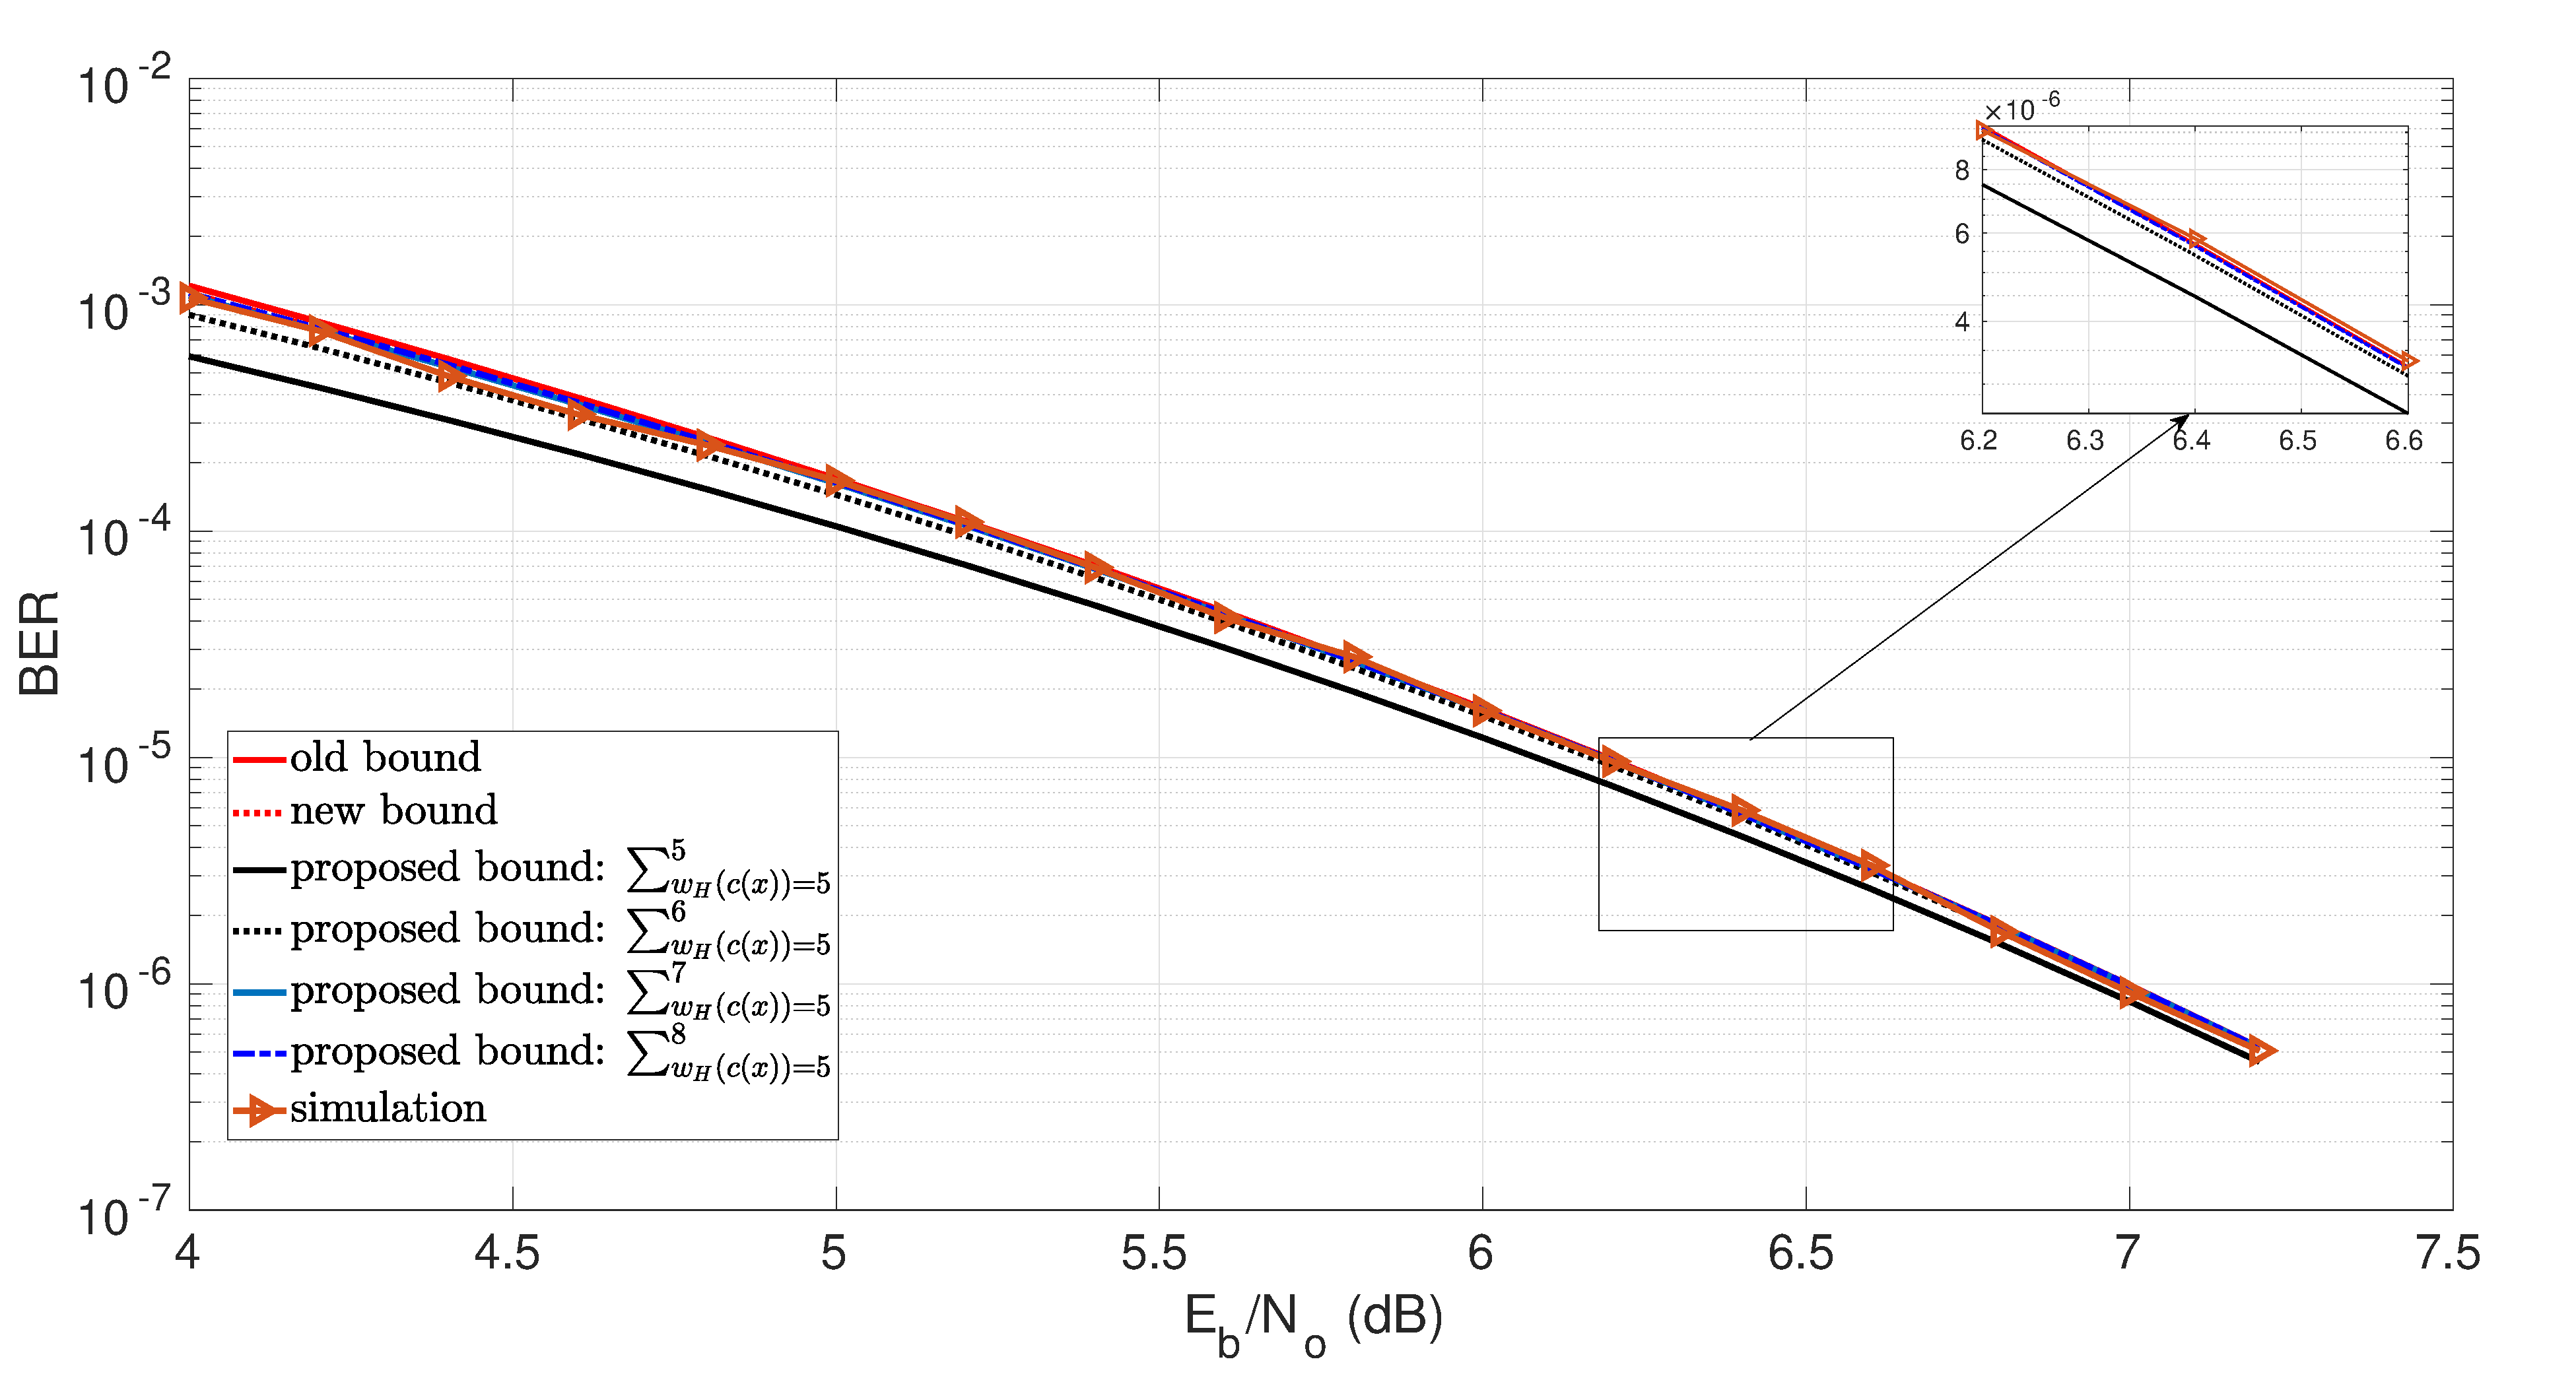
\includegraphics[width=1\textwidth]{./Images/RSC_5_7_lower_weights3.eps}
	\captionof{figure}{Old Bound vs New Bound vs Simulation for 5/7 RSC Code}
	\label{simFig1}
\end{figure}

As shown in Table \ref{code-tables-1}, since the free distance of the 5/7 RSC code is 5, and the codewords consisting of weigts 2 and 3 SCs or PCs are taken into account in the proposed method, all codewords with weights up to 7 are picked up. For the codewords of weight-8 on the other hand, some of them consisting of the weight-4 SC and PC are omitted in our method. However, Fig. \ref{simFig1} indicates that the union bound obtained using the codewords with weights up to $d_{\rm free+1}$ are sufficient to approximate the BER curve especially in the high-$E_b/N_0$ region. Moreover, the bounds obtained by our method and the transfer function converge to the same value with $E_b/N_0$ increament and match the simulation results. 

For the 37/21 RSC code, since the free distance of the code is 6, the counting omission in the proposed method occurs for the codewords higher than 7. Although Table \ref{code-tables-2} indicates that there are 3 weight-8 codewords, and only one of them is found by our method, we can see from Fig. \ref{simFig2} that their contributions to the union bound are negligible and the BER curve can be approximated using the codewords with weight 6 and 7 with a high accuracy at the high $E_b/N_0$ region.

\begin{figure}[htbp]
	\centering
	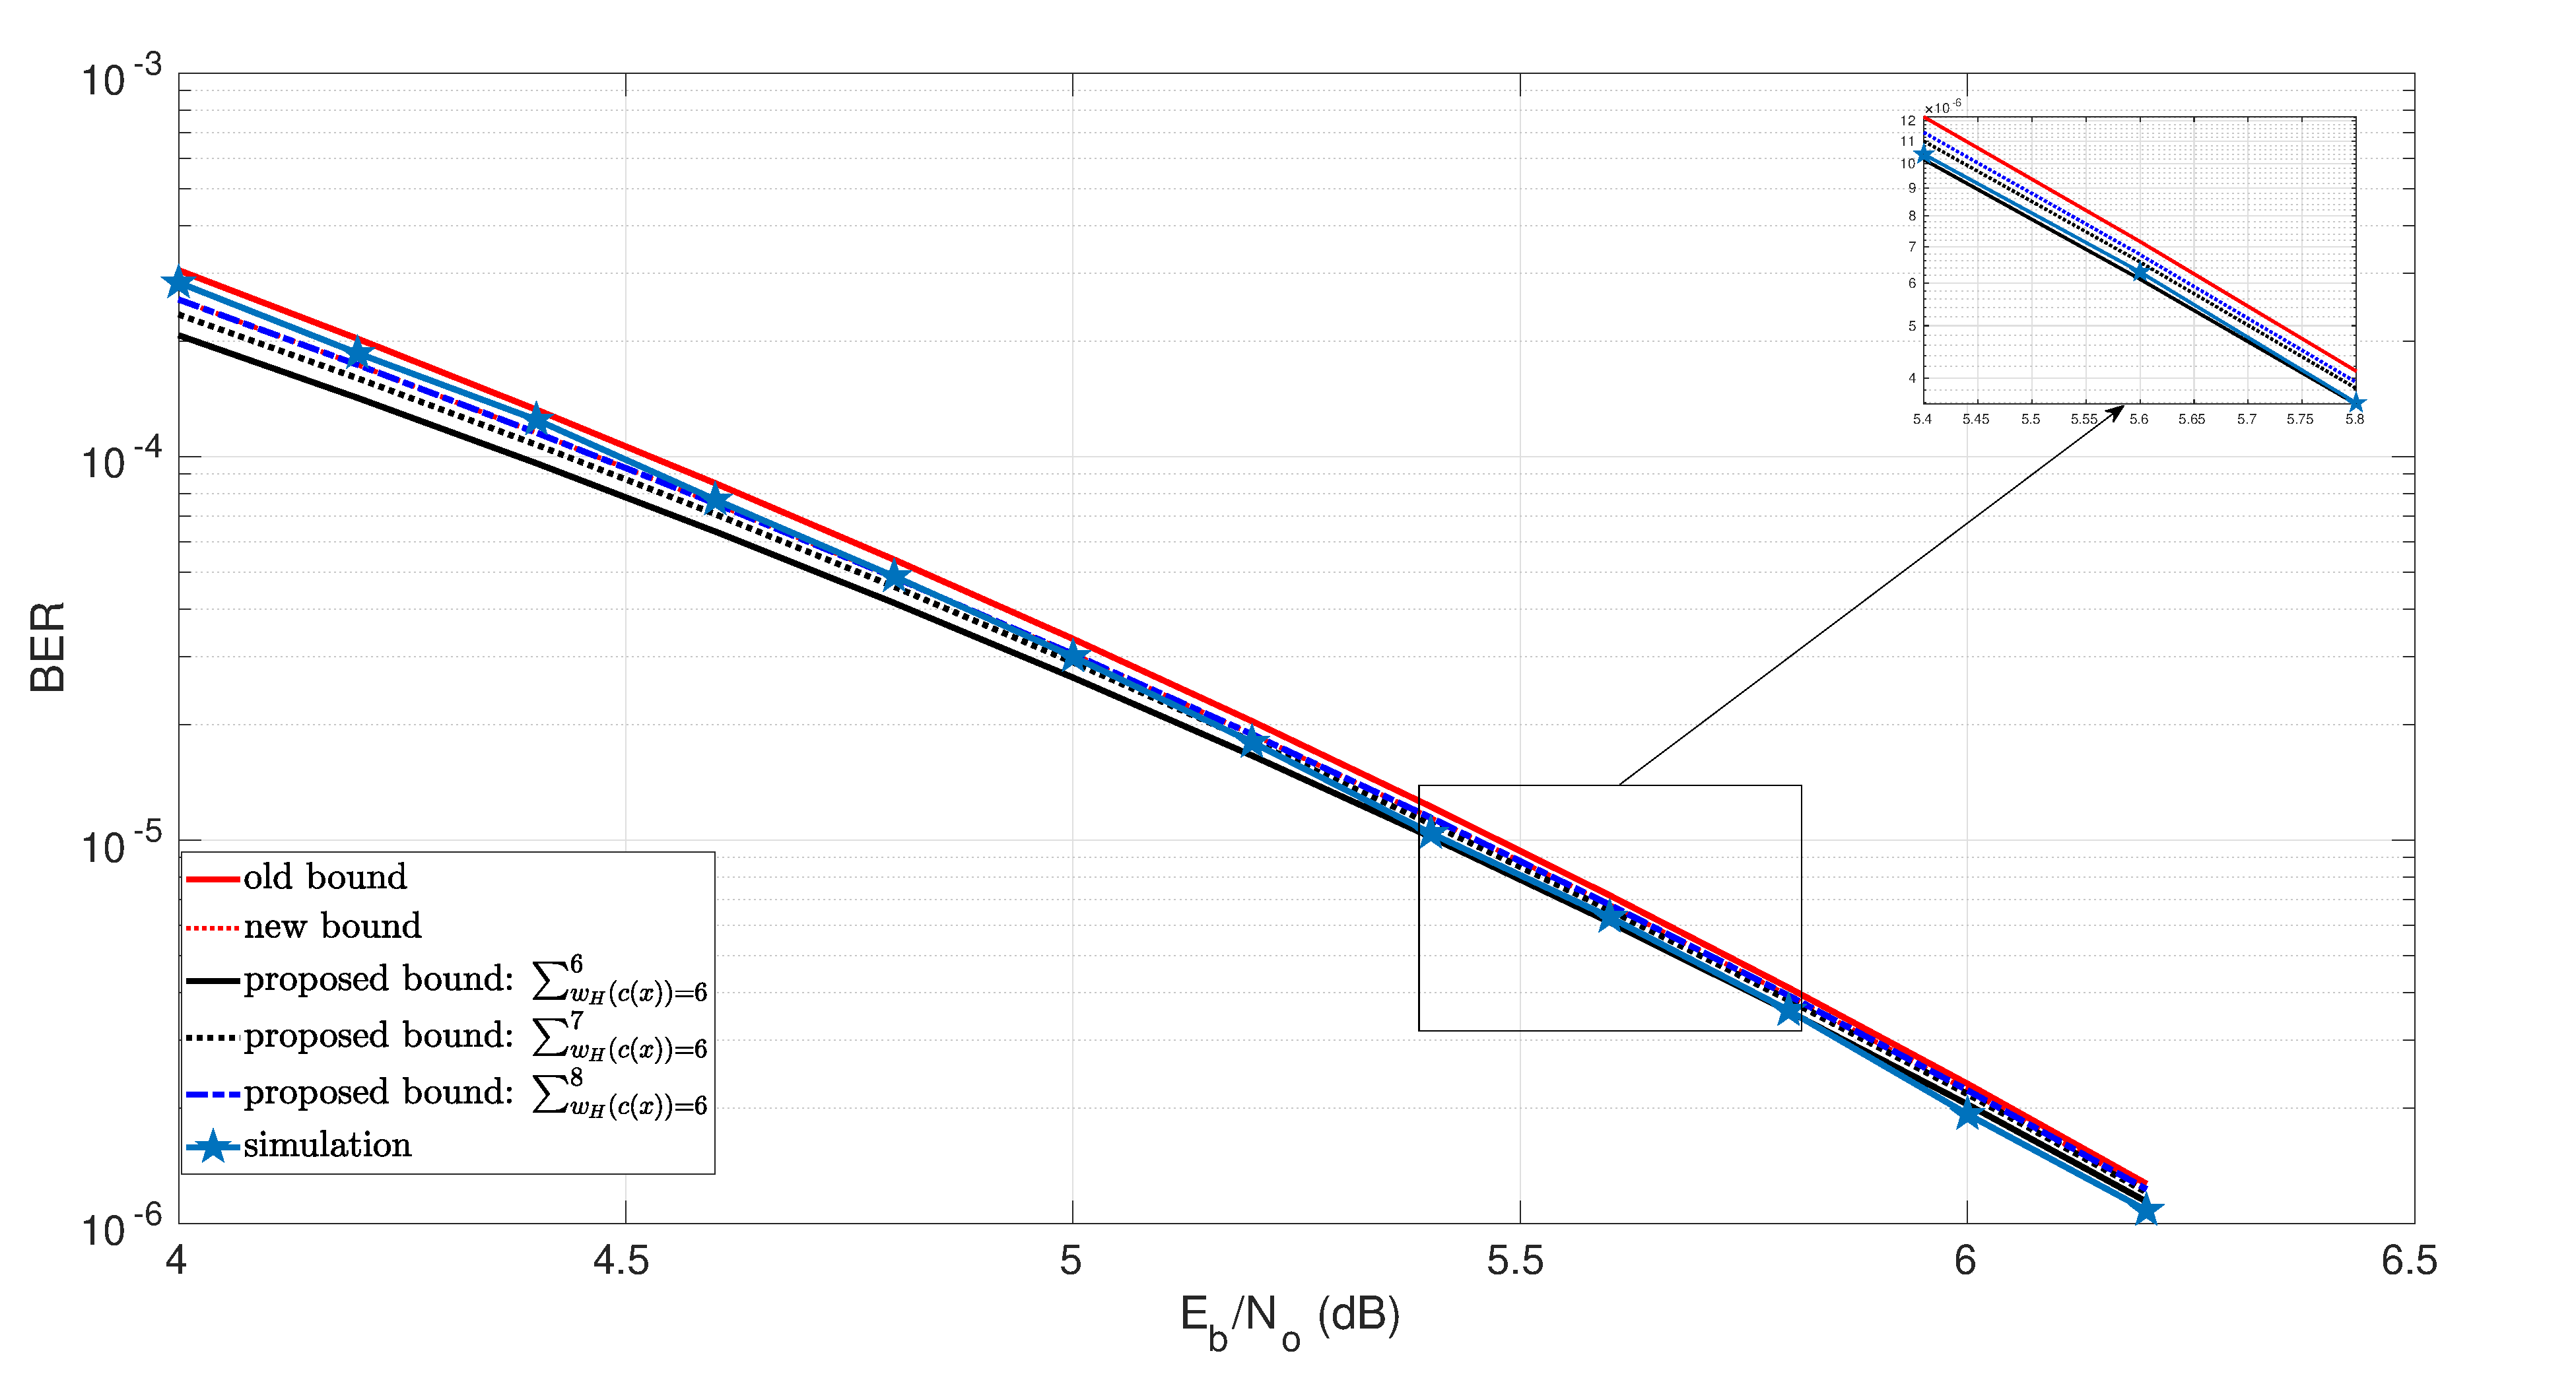
\includegraphics[width=1\textwidth]{./Images/RSC_37_21_lower_weights3.eps}
	\caption{Old Bound vs New Bound vs Simulation for 37/21 RSC Code}
	\label{simFig2}
\end{figure}

For the code III, the free distance is 7. Using the proposed method, we can identfy 2 codewords with weight-7 while 3 codewords with weight-8 can not be found as shown in Table \ref{code-tables-3}. Thus, while we use the weight-7 codewords to approximate the BER curve as Fig. \ref{simFig3}, there about 0.1 dB between the proposed method and simulation results.
%Even though it is possible to improve the accuracy of our proposed bound by considering SCs and PCs of weight-4. 

\begin{figure}[htbp]
	\centering
	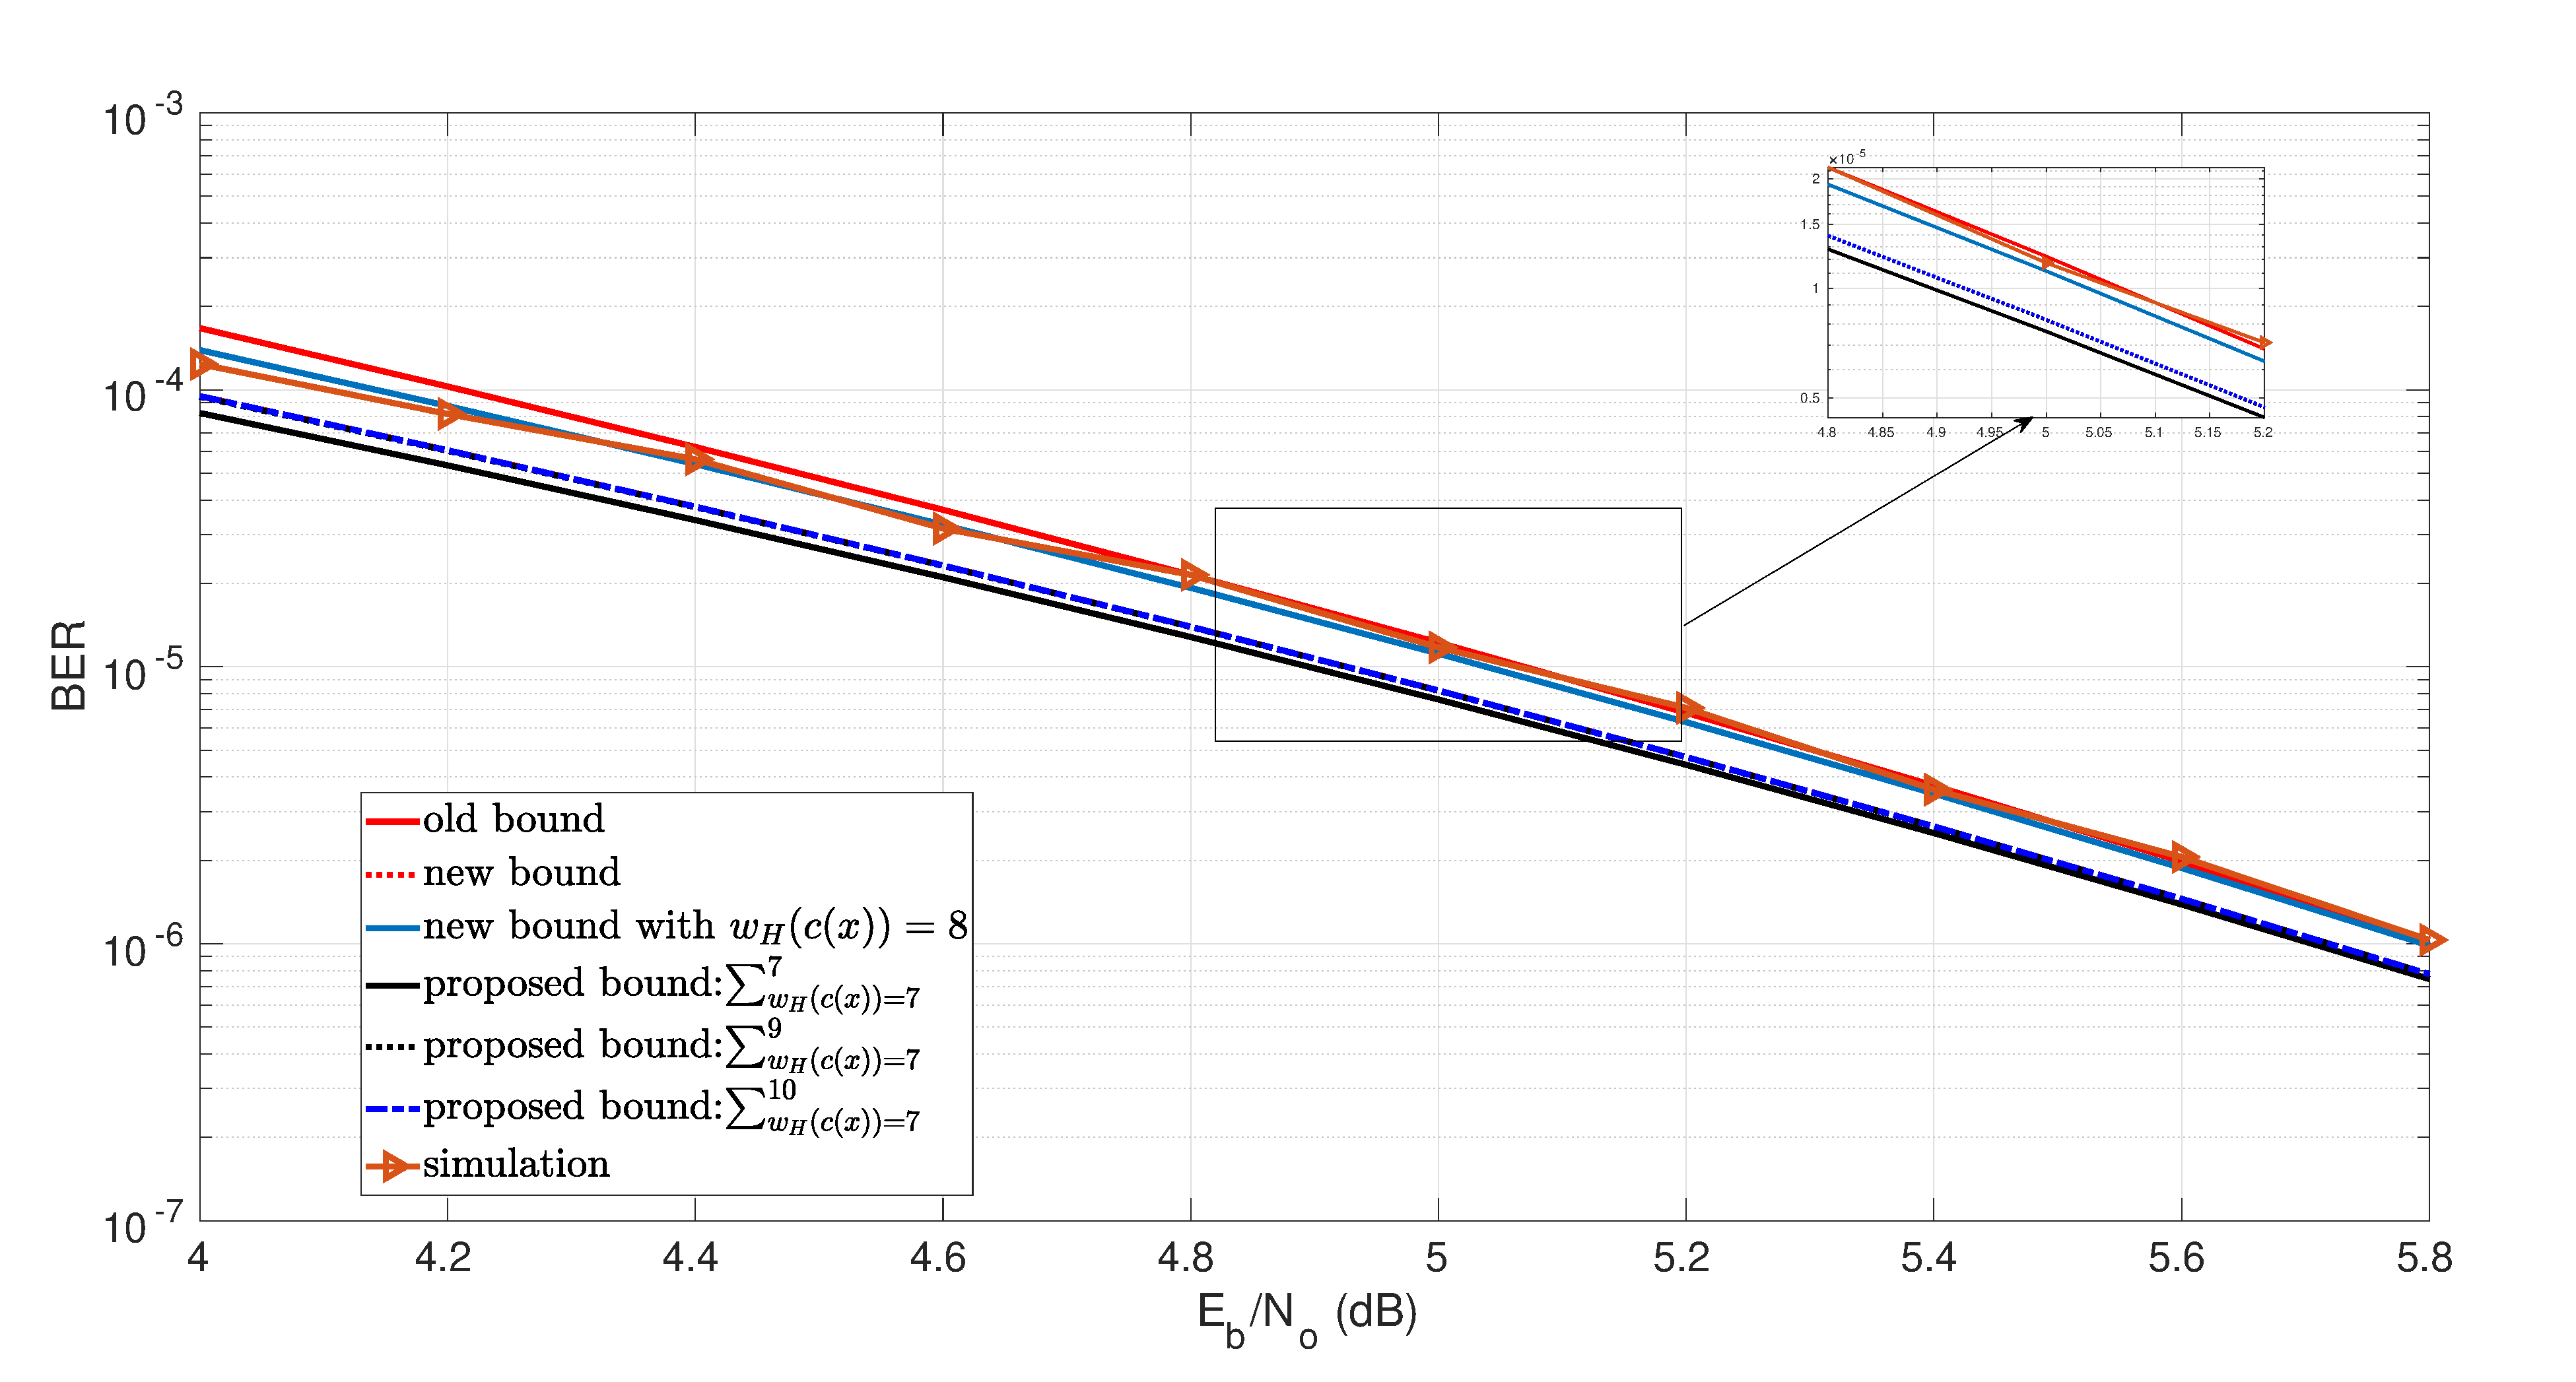
\includegraphics[width=1\textwidth]{./Images/RSC_23_35_lower_weights3.eps}
	\caption{Old Bound vs New Bound vs Simulation for 23/35 RSC Code}
	\label{simFig3}
\end{figure}

%\subsection{Discussion}
%
%We know from the previous discussion that take the codewords with weights $d_{\rm free}$ and $d_{\rm free +1}$ provides a good approximation of RSC code over AWGN channel. Now, we consider the code I-III from view point of interleaver design for Turbo code.
%
%For the code I, there 5 low-weight codewords 
%
%This means that when the 5/7 RSC code is used in a TC, the deterministic interleaver should be designed in such a way that it deals effectively with both weight-2 and weight-3 SCs. While, having to consider weight-3 SCs in the deterministic interleaver design introduces a bit of complexity, it is manageable since there is just a single $(m,n)$ pair that is associated with the weight-3 SCs.
%
%
%The fact that just a single $(m,n)$ pair needs to be considered for weight-3 SCs during interleaver design makes the 5/7 RSC code attractive for use in TCs.
%\label{ex-6}
%
%the added complexity as a result of considering weight-4 SCs in the interleaver design process makes this RSC code very unattractive for use in TCs.
%
%Given that weight-2 SCs and PCs are sufficient to derive the union bound, and deterministic interleaver design requires focusing on weight-2 SCs only, this RSC code is highly recommended for use in TCs.
%
%From Table \ref{novelTab15}, we observe that there are no weight-3 SCs. However, there exists weight-4 SCs that are not a combination of weight-2 SCs and when this RSC code is used in TCs, the deterministic interleaver needs to be designed to cater for weight-2 SCs as well as such weight-4 SCs. 



